
\chapter{DEEP LEARNING CHO BÀI TOÁN ĐẾM ĐỐI TƯỢNG TRONG ẢNH TĨNH.}
\ifpdf
    \graphicspath{{Chapter3/Chapter3Figs/PNG/}{Chapter3/Chapter3Figs/PDF/}{Chapter3/Chapter3Figs/}}
\else
    \graphicspath{{Chapter3/Chapter3Figs/EPS/}{Chapter3/Chapter3Figs/}}
\fi

\markboth{\MakeUppercase{\thechapter. DEEP LEARNING CHO BÀI TOÁN ĐẾM ĐỐI TƯỢNG.}}{\thechapter. DEEP LEARNING CHO BÀI TOÁN ĐẾM ĐỐI TƯỢNG.}
Trong chương này, sinh viên sẽ trình bày tổng quan các kiến thức nền tảng về máy học và Deep Learning (DL). cụ thể hơn trong phần 3.1 sinh viên sẽ trình bày sơ lược về các kiến thức như mô hình Neural Networks, tổng quan về Deep Learning và mô hình đang cực kỳ phát triển mang lại những kết quả rất đáng chú ý là mô hình Convolutional Neural Networks. Từ những kiến thức nền tảng đó, Sinh viên sẽ trình bày chi tiết về kiến trúc mô hình DL được đề xuất bởi Daniel và Roberto \cite{onoro2016towards} cho bài toán đếm đối tượng. Cụ thể đó là mô hình Counting CNN (CCNN) và mô hình cải tiến Hydra CNN. Từ kết quả thực nghiệm có thể nói đây là mô hình State-of-the-art cho bài toán đếm đối tượng.
\section{Tổng quan về Deep Learning.}
	

\subsection{Neural networks}
\subsubsection{Mạng neural nhân tạo.}
Mạng Neural nhân tạo (Artificial Neural Network: ANN), hay được gọi tắt là Neural Network là một mô hình xử lý thông tin được mô phỏng từ hoạt động của các hệ neural sinh học mà cụ thể hơn là não bộ của con người. Trong đó, thành phần cở bản của ANN là neural nhân tạo có các cách thức hoạt động và xử lý tương tự như neural sinh học. Do đó, để tìm hiểu về mạng neural nhân tạo, trước tiên ta sẽ tìm hiểu khái quát về mạng neural sinh học. \par
 	Cách thức hoạt động của bộ não nói riêng và cả hệ thần kinh nói chung đã được con người quan tâm nghiên cứu từ rất lâu. Nhưng cho đến nay, các nhà khoa học vẫn chưa thực sự hiểu rõ chi tiết về cách thức hoạt động của bộ não và hệ thần kinh con người. Đặc biệt là trong các hoạt động như ghi nhớ, suy nghĩ, học tập, sáng tạo, ... . Tuy nhiên, các nhà khoa học cũng đã thu được một số thông tin cơ bản về bộ não của con người. Theo đó, một bộ não của con người có khối lượng từ 1.2-1.4 kg hoặc khoảng 2\% tổng trọng lượng cơ thể với thể tích vào khoảng 1260 $cm^3$ ở nam và 1130 $cm^3$ ở nữ\footnote{$https://en.wikipedia.org/wiki/Human_brain$}. Cấu tạo bộ não chia thành nhiều vùng khác nhau và mỗi vùng đảm nhận một hay nhiều hoạt động của cơ thể con người. Quá trình hoạt động của hệ thần kinh bao gồm não bộ và các giác quan như sau: Khi con người tiếp nhận qua các giác quan từ những kích thích từ bên ngoài hoặc bên trong cơ thể. Các kích thích này được chuyển thành xung điện bởi chính các giác quan tiếp nhận nó. Những tính hiệu điện này được đưa về trung ương thần kinh, nơi bộ não sẽ tiến hành xử lý thông tin. Từ những hoạt động xử lý, đánh giá, so sánh với các thông tin đã được lưu trữ trước đây. Bộ não sẽ đưa ra quyết định được trả về dưới dạng xung điện. Các tính hiệu điện này sẽ được đưa đến các bộ phận thực thi đểu thực hiện các hành vi thích hợp như tay, chân, mắt, miệng hay các cơ, ... \par 
\begin{figure}[ht]
  \begin{center}
    \leavevmode
    \ifpdf
      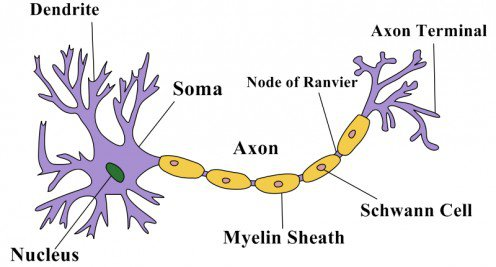
\includegraphics[scale=.7]{neural1}
    \else
      \includegraphics[scale=.7]{•}]{neural1}
    \fi
    \caption{Các thành phần cấu trúc của một neural nhân tạo\protect\footnote{https://owlcation.com/stem/Structure-of-a-Neuron}.}
    \label{FigAir}
  \end{center}
\end{figure}
 	  Khi xét ở mức độ tế bào thì bộ não được cấu thành từ $10^{11}$ phần tử gọi là nơ-ron (hay neural sinh học) và mỗi tế bào có thể kết nối với $10^4$ tế bào khác, nghĩa là có gần $10^{15}$ kết nối giữa chúng\footnote{https://en.wikipedia.org/wiki/Neuron}. Ngoài những đặc điêm chung có ở những tế bào khác thì chúng còn có khả năng nhận và xử lý các tính hiệu điện hóa. làm cơ sở cho việc hình thành cho việc xử lý thông tin của não bộ. Mỗi neural sinh học bao gồm 4 thành phần chính:
 	  \begin{itemize}
 	  	\item Thân neural(cell body) chưa nhân (nucleus) có nhiệm vụ chính là tổng hợp và xử lý các tín hiệu điện hóa từ các đầu vào. Thực chất quá trình này là việc lấy tổng của các tính hiệu mà neural nhận được.
 	  	\item Các dây dẫn (denrites) là các dây thần kinh truyền tính hiệu đến thân neural.
 	  	\item Sợi trục (axon) có chức năng truyền tín hiệu từ neural sang neural khác. Phần cuối của axon được chia thành những nhánh nhỏ kết thúc tại khớp nối (Synapse)
 	  	\item Khớp nối (Synapse) là điểm liên kết giữa sợi trục ra của neural này với các nhánh của neural khác. những liên kết giữa các neural và độ nhạy của mỗi Synapse được xác định bởi quá trình học phức tạp.
 	  \end{itemize}



\begin{figure}[ht]
  \begin{center}
    \leavevmode
    \ifpdf
      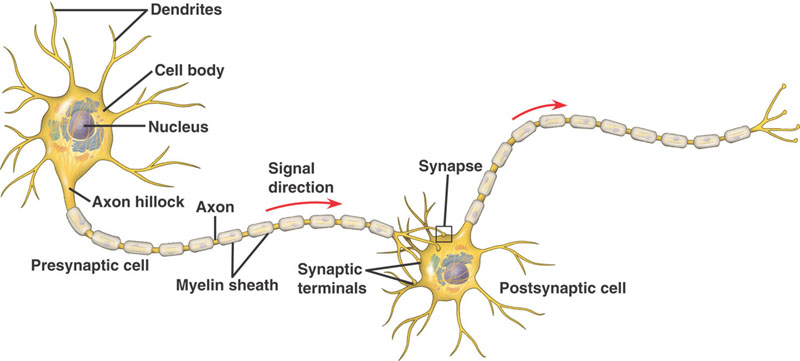
\includegraphics[scale=.5]{truyen}
    \else
      \includegraphics[scale=.5]{•}]{truyen}
    \fi
    \caption{mô hình kết nối và quá trình truyền tính hiệu giữa hai neural sinh học\protect\footnote{https://en.wikipedia.org/wiki/Neuron}. } 
    \label{FigAir}
  \end{center}
\end{figure}

	Một cách tổng quát, Neural sinh học hoạt động theo quy trình sau: neural nhận tính hiệu đầu vào từ các denrites. Sau đó nhân neural xử lý các tính hiệu này mà cụ thể là lấy tổng tất cả các tính hiệu chúng nhận được, sau đó phát ra một tính hiệu điện thế. Nếu giá trị điện thế lớn hơn một ngưỡng cho phép nào đó thì sẽ cho ra một tính hiệu đầu ra truyền ra các axon và chính là đầu vào của một neural khác. Dựa trên cấu trúc và cách hoạt động này thì các nhà nghiên cứu đã đề xuất ra mô hình neural nhân tạo hay Neural Networks.
	
	Mạng neural nhân tạo, là một mô hình tính toán được cấu thành từ nhiều phần tử tính toán gọi là neural được liên kết với nhau và cùng hoạt động song song. Một neural là một một đơn vị xử lý thông tin và là thành phần cơ bản cảu mạng ANN. Cấu trúc của một neural được mô tả trong hình \ref{neural} \par
	Trong đó: \par
	
	\begin{itemize}
		\item \textbf{Các giá trị đầu vào} Trong thực tế, những dữ liệu này thường được đưa vào dưới dạng một véc tơ N chiều.
		\item \textbf{Tập các liên kết:} Có chức năng truyền thôn tin. Trong đó một liên kết ứng với một trọng số (hay trọng số liên kết). Thông thường, các trọng số này được khởi tạo một cách ngẫu nhiên ở thời điêm ban đầu khởi tạo mạng và chúng được cập nhật liên tục trong quá trình học.
		\item \textbf{Hàm kết hợp:} Thường dùng để tính tổng từ các tham số đầu vào với trọng số liên kết tương ứng của nó (một số tài liệu còn gọi là hàm tổng - summing function).
	
		\[a_{k} = \sum_{i = 1}^nW_{ki}x_{i} + b_{k} \] 

		Với $W_{ki}$ là trọng số liên kết giữa các neural đầu vào và $b_{k}$ là ngưỡng hay độ lệch (bias).
		\item \textbf{Hàm truyền (transfer) hay hàm kích hoạt (active function):} Có chức năng để giới hạn phạm vi đầu ra của mỗi neural. Nó nhận đầu vào là kết quả của hàm kết hợp và ngưỡng đã cho. Thông thường, phạm vi đầu ra cảu mỗi neural được giới hạn trong đoạn [0,1] hoặc [-1,1]. Các hàm truyền rất đa dạng, có thể là hàm truyền tuyến tính hoặc phi tuyến (một số hàm truyền thường hay sử dụng được trình bay trong bảng \ref{bang1}). Việc lựa chọn hàm truyền thường phụ thuộc vào từng bài toán và kinh nghiệm cảu người thiết kế mạng. 
		\item \textbf{Đầu ra:} là tín hiệu đầu ra sau quá trình tính toán của một neural.
	\end{itemize}	

\begin{figure}[ht]
  \begin{center}
    \leavevmode

    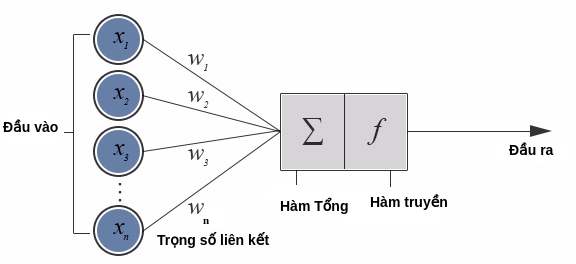
\includegraphics[scale=.7]{neuralart}
  
    \caption{Cấu trúc của một neural nhân tạo.} 
    \label{neural}
  \end{center}
\end{figure}

\begin{table}[!htp]
    \centering
    \begin{tabular}{|c|c|c|c|}
        \hline 
		\textbf{Tên Hàm Truyền}  & \textbf{Công Thức Toán Học} & \textbf{Đồ thị}\\ 
		\hline 
		Linear & f(x) = x  &  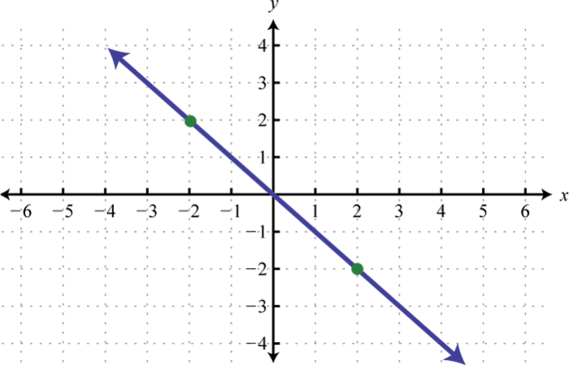
\includegraphics[scale=1]{linear} \\
		\hline 
		Tan-sigmoid & $ f(x) = \dfrac{ 1 - e^{x}}{1 + e^{x} } $ & 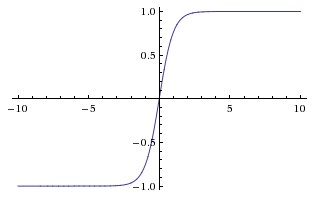
\includegraphics[scale=.5]{tan} \\
		\hline
		Sigmoid & $f(x)  \dfrac {1}{1 + e ^{-x} } $ & 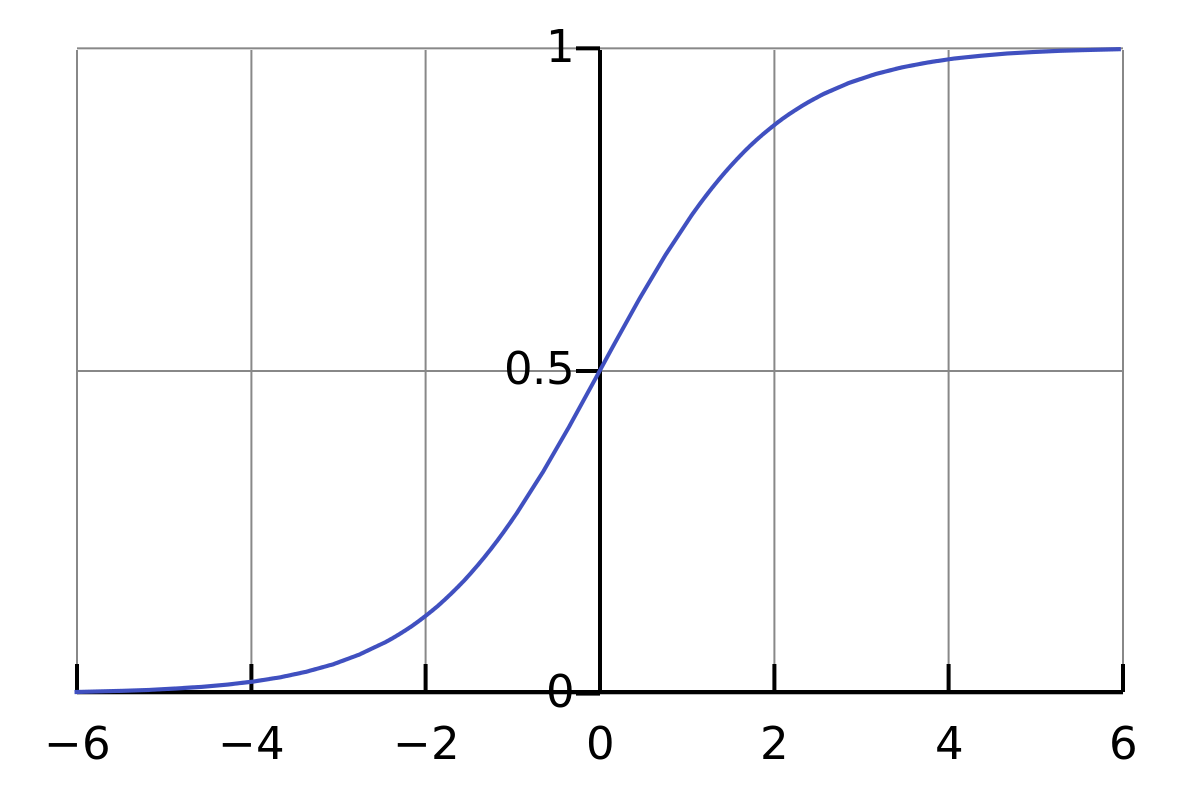
\includegraphics[scale=.15 ]{sig} \\
		\hline		
		ReLu & f(x) = max(0,x) & 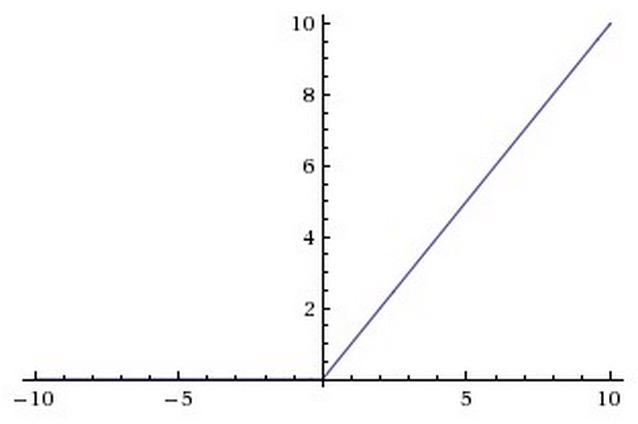
\includegraphics[scale=.3]{r} \\
		\hline
     \end{tabular}
    \caption{Một số hàm truyền thông thường sử dụng trong mạng neural}
    \label{bang1}
\end{table}

	Từ những neural máy tính này được kết hợp với nhau tạo ra một mạng ANN. Tính năng và cách hoạt động của mạng phụ thuộc hoàn toàn vào cấu trúc mạng, trọng số giữa các neural và quá trình xử lý trong mỗi đơn vị neural. Một mạng ANN bao gồm nhiều lớp (layer). Mỗi lớp bao gồm bao gồm nhiều neural có cùng chức năng. Dựa vào Số lớp và sự liên kết giữa các lớp trong mạng mà người ta phân loại ANN thành các nhóm khác nhau. \par
	\textbf{Phân loại dựa trên số lớp}
	Dựa theo số lớp trong mạng thì ANN được chia thành hai nhóm: mạng một lớp và mạng nhiều lớp.
	\begin{figure}[ht]
  			\begin{center}
    				
    				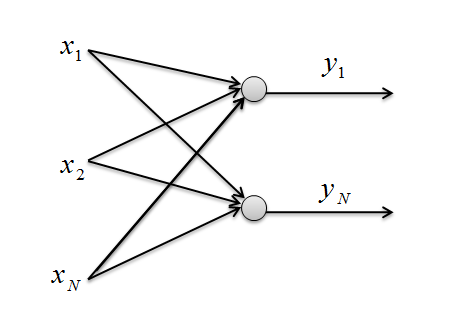
\includegraphics[scale=.6]{1layer}
    				\caption{Cấu trúc mô hình ANN 1 lớp.} 
    				\label{1layer}
  			\end{center}
		\end{figure}
	\begin{itemize}
		\item \textbf{Mạng một lớp:} Mạng một tầng tạo từ một lớp neural, nó vừa là tầng đầu vào vừa là tầng đầu ra của mạng.
		
		\item \textbf{Mạng nhiều lớp:} Đầy là một cấu trúc mạng ANN chứa n lớp ($n \ge 2$): trong đó gồm lớp nhận tín hiệu đầu vào (input). Các tín hiệu đầu ra của mạng được cho ra bởi lớp đầu ra của mạng - tần thứ n. Các lớp nằm ở giữa lớp vào và lớp ra được gọi là lớp ẩn - có (n-1) lớp ẩn.   
 	\end{itemize}
	
	\textbf{Phân loại dựa trên cách liên kết} \par
	Dựa theo cách liên kết giữa các thành phần trong mạng mà ta có thể chia ANN làm hai nhóm chính:
	\begin{itemize}
		\item \textbf{Mạng truyền thẳng} (feedforward neural networks): Đây là một mô hình đơn giản nhất của mạng neural.Các neural trong mạng truyển thẳng liên kết với nhau mà không có liên kết ngược (hay không hình thành nên chu trình). Tín hiệu sẽ truyền từ đầu vào, qua các lớp ẩn và đến đầu ra. Các neural trong cùng một lớp cũng không có liên kết với nhau. ()
\begin{figure}[ht]
  			\begin{center}
    				
    				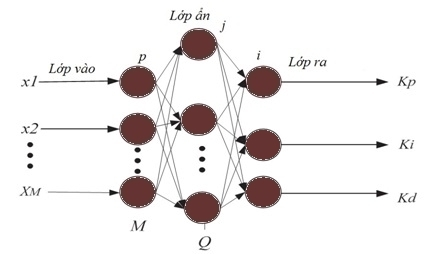
\includegraphics[scale=1]{nlayer}
    				\caption{Cấu trúc mạng nhiều tầng truyền thẳng.} 
    				\label{1layer}
  			\end{center}
\end{figure}
		\item \textbf{Mạng hồi quy} (recurrent neural network): Khác với mạng truyền thẳng. Mạng hồi quy chứa các liên kết ngược (hình thành nên chu trình). Mạng có khả năng lưu lại các trạng thái trước đó, và trạng thái tiếp theo không  chỉ phụ thuộc vào các tín hiệu đầu vào mà còn phụ thuộc vào các trạng thái đầu ra trước đó của nó. () 
	\end{itemize}
\subsubsection{Hoạt động của mạng neural nhân tạo.}
	Hoạt động của ANN có thể mô tả một cách cụ thể như sau: tại lớp đầu vào của mạng, các neural sẽ nhận tính hiệu xử lý (tính tổng từ tham số đầu vào và truyền kết quả đến hàm truyền) rồi cho ra kết quả (là kết quả cho ra từ hàm kích hoạt). Kết quả này sẽ được truyền tới các neural thuộc tần ẩn thứ nhất, các neural tại đây tiếp nhận các tính hiệu đầu vào rồi xử lý và lại gửi kết quả đến lớp ẩn thứ hai. quá trình này tiếp tục cho đến các neural lớp cuối cùng và cho ra kết quả.\par
	Chức năng của một mạng ANN được quyết định bởi các thành tố như: cấu trúc mạng (số lớp, số neural mỗi lớp và cách các lớp liên kết với nhau) và trọng số của các liên kết bên trong mỗi mạng. Kiến trúc mạng thông thường được dùng cố định cho mỗi bài toán và các trọng số liên kết được tính toán bởi các thuật toán huấn luyện mạng (traning algorithm). Quá trình điều chỉnh các trọng số để mạng có thể nhận biết được từ những dữ liệu đầu vào và cho ra kết quả dữ liệu đầu ra như mong muốn gọi là quá trình học (learning) hay huấn luyện (training).\par
	Để rõ hơn, giả sử ta có một tập huấn luyên (training set) $(x_{i},y_{i})$,..,$(x_{n},y_{n})$, với $x_{i}$ là dữ liệu đầu vào và giá trị mà ta mong muốn thu được sau quá trình tính toán là $y_{i}$. Ta gọi $y'_{i}$ là kết quả thu được thực tế thu được sau quá trình tính toán với đầu và $x_{i}$. Khi đó, bản chất của quá trình huấn luện là thay đổi các trọng số liên kết trong mạng thông qua các bộ huấn luyện sao cho $|y_{i} - y'_{i}|$ (sai số) là nhỏ nhất. Một trong những phương pháp huấn luyện ANN là phương pháp lan truyền ngược (Backpropagation). \par
	Backpropagation là thuật toán huấn luyện mạng thường được sử dụng với một phương pháp tối ưu, Điển hình là phương pháp Gradient  Descent. Phương pháp Gradient Descent được phát triển dựa vào hướng tăng lớn nhất (gradient) tại điểm x thuộc hàm f(x). Gradient tại x của hàm f(x) được tính bởi đạo hàm theo công thức: $\dfrac{\partial{f}}{\partial{x}}$. Gradient tại x sẽ cho biết hướng làm cho hàm f(x) sẽ đạt cực đại. nếu đi ngược lại hướng đó, ta sẽ thu được điểm cực tiểu của hàm. Từ ý tưởng đó, thuật toán Gradient Descent ra đời. \par
	Thuật toán lan truyền ngược sẽ điểu chỉnh các trọng số sao cho thu được bộ giá giá trị tối ưu nhất (đạt sai số thấp nhất). Lúc ban đầu, ANN sẽ được khởi tạo tập trọng số và tham số học tập $ \alpha $ (learning rate). Tập trọng số sẽ được gán ngẫu nhiên và thường là những giá trị nhỏ (trong khoảng $[-1,1]$). Learning rate là tham số để kiếm soát sự thay đổi của các tham số trong mạng và giúp hàm đạt độ lỗi cực tiểu sau quá trình huấn luyện. Nếu giá trị của $\alpha$ nhỏ, thì giá trị thay đổi trọng số ít và quá trình huấn luyện lâu. Nếu giá trị lớn thì sẽ gây ra hiện tượng sai số vì trọng số thay đổi ở mỗi bước quá nhiều. Do vậy, hiện nay chưa có một kỹ thuật nào có thể tối ưu được việc chọn tham số học tập mà chủ yếu dựa vào thực nghiệm. \par   	
	Quá trình học mạng bao gồm hai giai đoạn chính được lặp đi lặp lại gồm: \textbf{lan truyền} và \textbf{Cập nhật trọng số}. \par
	\begin{itemize} 
	\item \textbf{Lan truyền}: trong giai đoạn được chia làm hai quá trình.
	\begin{itemize}
		\item Từ bộ dữ liều đầu vào, chúng đi qua hàm kích hoạt và bộ trọng số được khởi tạo ban đầu để xác định giá trị cho các lớp neural tiếp theo. Cho đến khi thu được giá trị đầu ta của lớp neural cuối cùng. 
		\item Từ giá trị thu được sau cùng, Ta tính toán được sai số ở đầu ra và sau đó lan truyền ngược từ lớp đầu ra đến lớp đầu tiên để tính toán gradient tại các lớp ẩn trong mạng.
	\end{itemize}
	\item \textbf{Cập nhật trọng số:} là quá trình điểu chỉnh trọng số theo giá trị $\alpha$ và giá trị gradient đã tính toán trong quá trình lan truyền ngược.
	\end{itemize}
	 Nói tóm lại, Việc huấn luyện cho mạng ANN là bài toán xác định các trọng số liên kết trong mạng sao cho sai số đầu ra là nhỏ nhất.\par
\subsection{Tổng quan deep learning}
	Deep Learning (DL) đang là một chủ đề đang thu hút rất nhiều sự quan tâm từ các nhà nghiên cứu cũng như các hãng công nghệ lớn trên thế giới. bởi lý do DL đã thu được  những kết quả hết sức nổi bật so với các phương pháp trước đây. Ví dụ như với bài toán phân lớp ảnh trên tập dữ liệu Imagenet \footnote{http://image-net.org/}, Nhờ áp dụng DL mà độ lỗi thu được đã giảm từ $ 28\% $ năm 2010 xuống còn $ 4,82\% $ năm 2015. Kết quả này thậm chí còn tốt hơn người với độ lỗi là $ 5,1\% $. Không dừng lại ở đó, DL còn đạt được những kết quả ấn tượng trong các cuộc thi như phát hiện đối tượng, nhận diện biển báo giao thông ... và áp dụng trong nhiều lĩnh vực như Xử lý tiếng nói(Spoken Language Processing), xử lý ngôn ngữ tự nhiên(natural language processing - NLP). \par
	
	Theo Li Deng and Dong Yu  và LISA Lab, hiện nay có một vài định nghĩa cho Deep Learning như sau: \par
	
	\begin{itemize}
		\item \textbf{Định nghĩa 1:} “Deep Learning là một phần của máy học dựa trên việc học qua nhiều cấp độ, tương ứng với hệ thống các đặc trưng hoặc các khái niệm. Những khái niệm ở cấp cao hơn được xây dựng từ khái niệm ở cấp thấp và những khái
niệm cùng cấp có thể dùng để định nghĩa những khái niệm cấp cao hơn.”
		\item \textbf{Định nghĩa 2:} “Deep Learning là một nhánh của máy học bao gồm tập các thuật toán nhằm trừu tượng hóa mô hình dữ liệu bậc cao bằng cách sử dụng nhiều lớp xử lý với cấu trúc phức tạp, được tạo nên bởi các mô hình biến đổi phi tuyến.”
		\item \textbf{Định nghĩa 3:} “Deep Learning là tập hợp các kỹ thuật máy học khai thác nhiều lớp xử lý thông tin phi tuyến nhằm biến đổi và trích xuất đặc trưng giám sát hoặc không giám sát, và phục vụ cho phân tích mẫu và phân loại.”
		\item \textbf{Định nghĩa 4:} “Deep Learning là hướng nghiên cứu mới của lĩnh vực Máy Học, được phát triển với mục đích mang Máy Học tiến gần mới mục đích ban đầu của nó: Trí Tuệ Nhân Tạo. Deep Learning trừu tượng hóa nhiều cấp độ của dữ liệu và giúp tìm ra ý nghĩa ẩn chứa trong dữ liệu.”
	\end{itemize}
	Từ đó, một cách tổng quát DL là một khái niệm chỉ các thuật toán máy học dựa trên ANN để xây dựng mô hình hay phát hiện ra các quan hệ phức tạp trong dữ liệu bằng những phương pháp học theo nhiều tầng. Kết quả của tầng trước là dữ liệu đầu vào cho tầng kế tiếp, mô hình được học ở tầng sau có tính tổng quát hơn so với mô hình trước. \par
\begin{figure}
  			\begin{center}
    				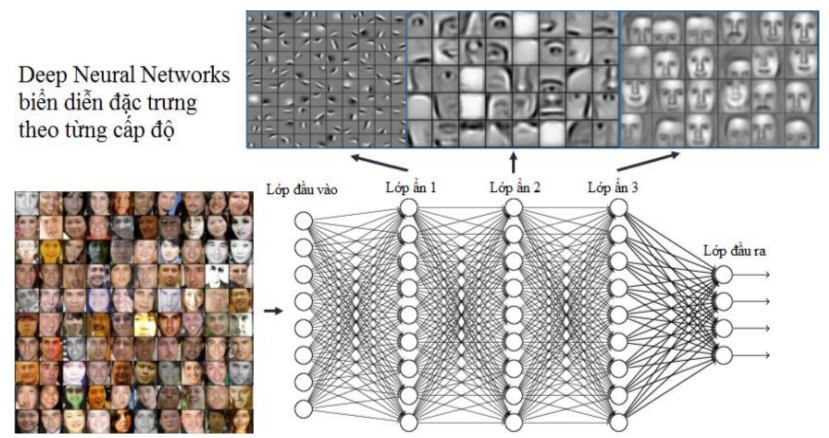
\includegraphics[scale=0.5]{DL1}
    				\caption{Các đặc trưng trên khuôn mặt từ tập dữ liệu sẽ được học qua quá trình huấn luyện. các lớp sau có thể tổng hợp và từ dữ liệu đầu ra của lớp trước đó cho ra những đặc trưng tổng quát và phức tạp hơn.} 
    				\label{DL1}
  			\end{center}
\end{figure}		
	Các kiến trúc cảu Deep Learning có khác biệt so với kiến trúc của ANN thông thường là bởi vì chiều sâu hay số lớp của chúng. Một ví dụ cho Deep Learning là mô hình cấu trúc Deep Neural Networks (DNNs). DNNs thông thường sẽ có số lớp ẩn nhiều hơn so với ANN.Trong Deep Learning, mỗi lớp sẽ đống vai trò huấn luyện một đặc trưng nhất định dựa vào đầu ra của lớp trước đó. Các lớp càng về sau sẽ học được các thông tin quan trọng hơn và càng mang tính tổng quát được tổng hộp từ những lớp trước đó. Có thể biểu nói DL là mô hình tự học các đặc trưng theo từng cấp bậc (feature hierarchy). Đặc trưng được tự học qua quá trình huấn luyện DL. Đặc trưng ở mức càng cao thì độ phức tạp và tính tổng quát càng cao (hình \ref{DL1} là một ứng dụng minh họa trong việc áp dụng Deep Neural Networks cho bài toán nhận dạng khuôn mặt). \par

	Đối với các mô hình DL với số lượng lớp lớn, thì lượng tham số có thể lên đến hàng tỷ tham số. Điều này làm cho DL phức tạp hơn rất nhiều và có khả năng xử lý lượng dữ liệu lớn. Ngoài ra, Deep Learning có khả năng xử lý trên cả dữ liệu không gián nhãn (unlabeled) và cả giữ liệu không có cấu trúc (unstructured data). Đối với dữ liệu không có cấu trúc, Deep Learning cho phép tìm ra những thông tin hoặc cấu trúc bị từ dữ liệu huấn luyện. Với dữ liệu không gián nhãn, thì DL sẽ liên tục tiến hành tái cấu trúc đầu vào tại đầu ra của mạng và so sánh với dữ liệu huấn luyện nhằm cố gắng cực tiểu hóa độ sai lệch giữa chúng. \par   
	 Từ những phương pháp huấn luyện khác nhau, ta có thể phân lại Deep Learning thành ba nhóm cơ bản: Deep Learning cho học có giám sát, Deep Learning cho học không giám sát và Hybird Deep Learning - Deep Learning có kết hợp cả hai phương pháp học có giám sát và không giám sát. \par
	 
	 \textbf{Deep Learning cho học có giám sát (Supervised Learning).} Là một phương pháp trong máy học với mục đích nhằm tạo ra một mô hình có khả năng dự đoán kết quả từ một tập dữ liệu đã được gán nhãn. Tập dữ liệu chứa các mẫu dữ liệu huấn luyện, mỗi mẫu huấn luyện có cấu trúc là một cặp giá trị đầu vào và các nhãn tương ứng. Thuật toán học có giám sát sẽ tiến hành học từ tập dữ liệu được gán nhãn tạo ra một mô hình hoàn chỉnh và từ mô hình đó để áp dụng xử lý cho những mô hình mới. Chức năng chủ yếu của phương pháp học có giám sát đó là giải quyết các bài toán phân lớp (Classification) và toàn toán hồi quy (Regression). \par
	 Trong Deep Learning, Phương pháp học có giám sát chủ yếu sẽ được áp dụng để giải quyết hai nhóm bài toán chính đó là bài toán nhận dạng và bài toán dự đoán. Dưới đây sinh viên sẽ giới thiệu hai kiến trúc Deep Networks nổi bật nhất trong phương pháp học có giám sát là Deep Neural Networks và Convolutional Neural Networks.
\begin{itemize}
	\item \textbf{Deep Neural Networks (DNNs):} Là một phiên bản mô hình mạng neural nhiều lớp của một ANN truyền thống. Các lớp trong Deep Neural Networks kết nối với nhau theo kiểu fully-connected, tức là một neural ở lớp này sẽ kết nối tới toàn bộ các neural ở lớp tiếp theo. Điều này sẽ dẫn đến số lượng liên kết neural rất lớn. Vì kiến trúc đa lớp nên việc huấn luyện sẽ khó khăn và phức tạp hơn so với các mô hình ANN truyền thống. 
\begin{figure}[t]
  			\begin{center}
    				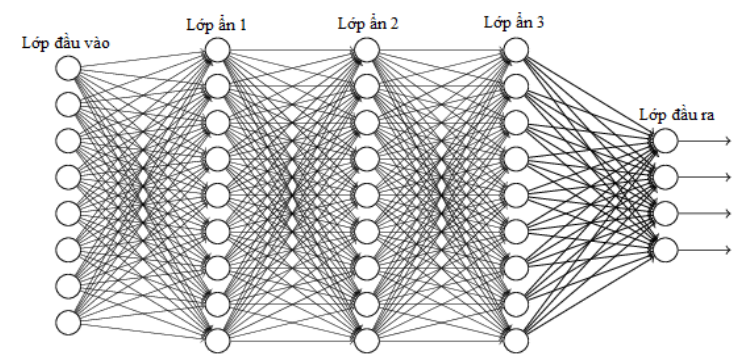
\includegraphics[scale=0.6]{ANNs}
    				\caption{Minh họa mô hình Deep Neural Networks với ba lớp ẩn, một lớp đầu vào và một lớp đầu ra với cùng kiểu liên kết fully-connected.} 
    				\label{ANNs}
  			\end{center}
\end{figure}	

	\item \textbf{Convolutional Neural Networks (CNN):} hiện tại là thuật toán đang cho kết quả tốt nhất trên các bài toán thuộc lĩnh vực thị giác máy tính. Hình \ref{CNN_chu} là một ví dụ về việc sử dụng CNN cho bài toán nhận diện chữ viết tay mang tên LeNet5 được phát minh bởi giáo sư Yan LeCun năm 1998. Mô hình LeNet5 được huấn luyện trên tập MNIST \footnote{$http://yann.lecun.com/exdb/mnist/$} và có sai số rất nhỏ (gần $1\%$). Lý thuyết và những thành phần cụ thể của mô hình CNN sẽ được trình bày trong phần tiếp theo của chương này. 
	
\begin{figure}[t]
  			\begin{center}
    				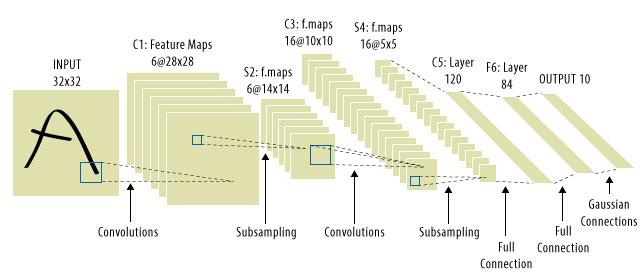
\includegraphics[scale=0.6]{CNN_chu}
    				\caption{Minh họa mô hình CNN sử dụng cho bài toán nhận dạng chữ viết tay.} 
    				\label{CNN_chu}
  			\end{center}
\end{figure}	

\end{itemize}	  
	 

\textbf{Deep Learning cho học không giám sát (Unsupervised
Learning):} là kỹ thuật học từ dữ liệu không được dán nhãn. Mục đích của học không giám sát là tìm ra các thông tin hoặc cấu trúc bị ẩn dưới dữ liêu.\par
Trong Deep Learning, các mô hình học không giám sát thường được áp dụng để giải quyết các bài toán như gom nhóm dữ liệu, phát hiện bất thương, hay khởi tạo trọng số cho các mô hình học có giám sát. Một số thuật toán DL tiêu biểu cho việc học không giám sát đó là Deep Belief Networks (DBNs) hay Deep Autoencoders (DAs). Dưới đây sẽ trình bày sơ lược về kiến trúc của 2 thuật toán này. 
\begin{itemize}
	\item \textbf{Deep Belief Networks (DBNs):} có thể đỉnh nghĩa như một cấu trúc chứa nhiều mạng Restricted Boltzmann Machine (RBMs) \footnote{$https://en.wikipedia.org/wiki/Restricted_Boltzmann_machine$}. Các lớp ẩn của các RBMs sẽ là lớp đầu vào cảu RBMs tiếp theo trong mạng DBNs. Cộng việc huấn luyện DBNs rất phức tạp và tốn nhiều thời gian hơn so với các kiến trúc DL khác. DBNs được huấn luyện bằng cách huấn luyện từng RBMs thành phần. Kết quả đầu ra của RBMs đầu tiên sẽ làm đầu vào cho RBMs tiếp theo. 
\begin{figure}[t]
  			\begin{center}
    				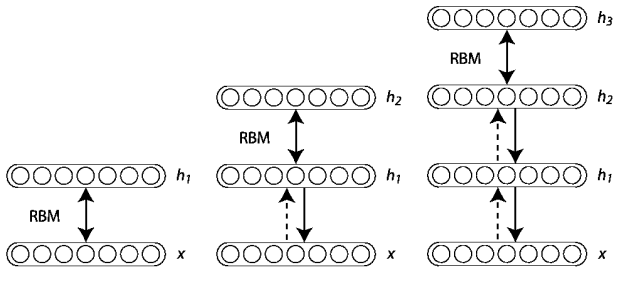
\includegraphics[scale=0.6]{DBNs}
    				\caption{Minh họa kiến trúc mô hình Deep Belief Networks (DBNs).} 
    				\label{CNN_chu}
  			\end{center}
\end{figure}		

	\item \textbf{Deep Autoencoders (DAs): } phát trển dựa trên mô  hình autoencoder - mô hình mạng neural được huấn luyện bằng thuật toán lan truyền ngược mà trong đó không sữ dụng dữ liệu được gián nhãn mà thực hiện bằng cách cho giá trị đầu ra bằng giá trị đầu vào. hay nói các khác là tìm một hàm xấp xỉ sao cho đầu ra bằng đầu vào.
\begin{figure}[t]
  			\begin{center}
    				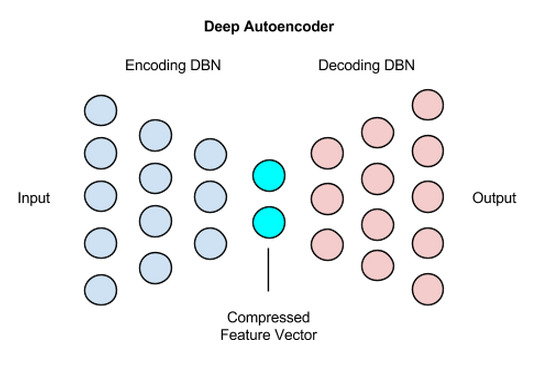
\includegraphics[scale=0.8]{DAs}
    				\caption[Caption for LOF]{Minh họa kiến trúc mạng DAs\protect\footnotemark} 
    				\label{CNN_chu}
  			\end{center}
\end{figure}		
\footnotetext{$https://deeplearning4j.org/deepautoencoder$}
\end{itemize}

\textbf{Hybird Deep Learning (HDLs)} hay còn được gọi với một tên khác là mô hình Deep Learning "lai". Mô hình này kết hợp cả hai phương pháp học có giám sát (Supervised Learning) và học không giám sát (Unsupervised Learning) nhằm mục tiêu nâng cao độ chính xác. Cụ thể hơn, trong huấn luyện mạng thường sử dụng mô hình học không giám sát để tiến hành khởi tạo các trọng số cho mô hình học có giám sát. Ví dụ như ta có thể sử dụng DBNs để khởi tạo trọng số cho mô hình CNN. Khi đó, ta nói răng mô hình kết hợp DBN-CNN là mô hình HDLs. 
 
\subsection{Convolutional Neural Networks}
	CNN là một trong những thuật toán DL cho kết quả tốt nhất hiện nay trong hầu hết các bài toán về thị giác máy tính. Nó là một kiểu của mạng neural nhân tạo với các kết nối giữa các neural được lấy ý tưởng dựa trên sự tổ chức của các neural trong vỏ não thị giác của động vật. Vào năm 1968, hai nhà thần kinh học \textbf{Hubel}\footnote{$https://en.wikipedia.org/wiki/David\_H.\_Hubel$} và \textbf{Wiesel}\footnote{$https://en.wikipedia.org/wiki/Elie\_Wiesel$} đã tìm ra rằng, trong vỏ não thị giác của động vật có chứa các cấu trúc thần kinh phức tạp. Nó chịu trách nhiệm phát hiện ra ánh sáng tại những vùng nhỏ chồng chéo của vùng thị giác (visual field) những vùng này còn được gọi là vùng tiếp nhận (receptive fields). Từ ý tưởng đó, CNN cũng 	chứa nhiều lớp neural với những vùng kết nối giữa hai lớp neural với nhau.Điều này giúp cho CNN tìm ra những thể hiện tốt hơn. Về cơ bản, CNN là một kiểu mạng ANN truyền thẳng với kiến trúc chính gồm nhiều thành phần được ghép nối với nhau theo cấu trúc lớp bao gồm: Convolution, Pooling, ReLU và Fully connected. Trong phần này sẽ trình bày chi tiết về các thành phần của CNN.

\subsubsection{Lớp Convolution}
Tầng Convolution (Conv) là tầng quan trọng nhất trong kiến trúc của CNN. Conv dựa trên lý thuyết xử lý tính hiệu số, việc lấy tích chập sẽ giúp trích xuất được những thông tin quan trọng từ dữ liệu. Conv hoạt động dựa trên đầu vào được biểu diễn bằng một ma trận hai chiều. Ta có thể hình dung phép tính này được thực hiện bằng cách dịch chuyển một cửa sổ mà ta gọi là kernel trên ma trận đầu vào. Trong đó, kết quả trước khi mỗi lần dịch chuyển được thu được bằng cách tính tổng tích chập (tích của các giá trị giữa hai ma trận tại vị trí tương ứng), sau khi trượt qua hết toàn bộ ma trận đầu vào, kết quả cho ra một ma trận kết quả có kích thước bé hơn hoặc bằng ma trận đầu vào. Kerne sẽ được sinh ra sau quá trình huấn luyện để có thể trích xuất ra những đặc trưng phù hợp nhất với yêu cầu bài toán. \par
\begin{figure}[ht]
  			\begin{center}
    				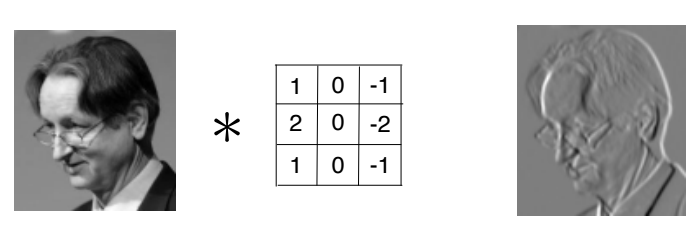
\includegraphics[scale=0.6]{Conv}
    				\caption[Caption for LOF]{minh họa cho việc tính tích chập với ảnh đầu vào ở bên trái, ở giữa là ma trận tích châp (kernel) và bên phải là đặc trưng thu được  (feature map)} 
    				\label{Conv}
  			\end{center}
\end{figure}	
	Khi áp dụng phép tính Conv cho xử lý hình ảnh, Người ta nhận thấy rằng Conv sẽ giúp biến đổi các thông tin đầu vào thành các yếu tố đặc trưng (nó tương tự như bộ phát hiện nhằm phát hiện ra các đặc trưng như cạnh, hướng, ...). Hình \ref{Conv} minh họa cho việc áp dụng phép tính Conv trên ảnh và cho ra kết quả là một feature map. Cụ thể hơn, Conv sẽ trích xuất đặc trưng của ảnh đầu vào qua các vùng ảnh nhỏ. Các vùng này được gọi là Local Receptive Field (LRF). Tích chập sẽ tính toán trên các LRF chồng lấp lên nhau. Độ chồng lắp này phụ thuộc vào hệ số trượt S (stride) của từng kiến trúc mạng cụ thể. Nếu sử dụng với hệ số trượt S = $\alpha$, thì tương ứng LRF (bằng kích thước với kernel) sẽ dịch chuyển $\alpha$ đơn vị pixel sau mỗi lần tích chập.  \par

\begin{figure}[ht]
  			\begin{center}
    				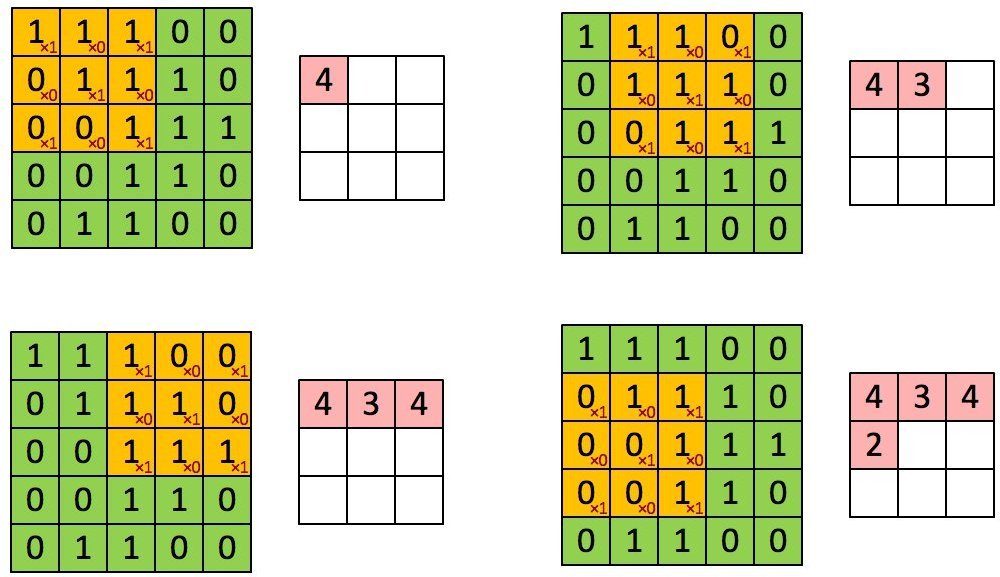
\includegraphics[scale=0.4]{con4}
    				\caption[Caption for LOF]{minh họa quá trình tính toán Conv với hệ số trượt bằng 1.} 
    				\label{Conv4}
  			\end{center}
\end{figure}	

	Ảnh đầu vào sau khi thực hiện quá trình tích chập sẽ thu được feature map, số LRF ở ảnh đầu vào sẽ tương ứng với số neural ở feature map và kernel sẽ là trọng số liên kết mỗi LRF với một neural ở feature map. Lớp conv có thể chứa một hoặc nhiều feature map. Nếu lớp conv có K feature map, thì ta nói lớp conv này có độ sâu là k.
	Để hình dung rõ hơn về quá trình này, sau đây sẽ minh họa quá trình trích xuất đặc trưng từ ảnh đầu vào cụ thể như sau: thực hiện xử lý tính giá trị đầu ra của một  ảnh có kích thước $W_1 \times H_1 \times D_1$ ($W_1$ và $H_1$ lần lượt là chiều rộng và chiều cao của ảnh và $D_1$ là chiều sâu hay thực chất là giá trị tại 3 kênh màu tương ứng của ảnh RGB). khi đó, một Conv như một cửa sổ trượt (sliding window, còn được gọi là kernel, filter hay feature detector) với kích thước $F \times F$ - giả sử trong trường ta sử dụng K filter. Trong quá trình xử lý, mỗi filter sẽ được tính toán với tất cả các LRF trong hình và $S = \alpha$. Trong một số trường hợp để cân bằng giữa số bước di chuyển và kích thước của ảnh, người ta đã chèn thêm P pixel với một giá trị màu được gán (thông thường là 0) xung quanh viền của ảnh. sau cùng ta thu được ma trận đầu ra (feature map) với kích thước $W_2 \times H_2 \times D_2$ với giá trị cụ thể như sau: \par
	\begin{itemize}
		\item $W_2 = \frac{(W_1 - F + 2P)}{\alpha} + 1$
		\item $H_2 = \frac{(H_1 - F + 2P)}{\alpha} + 1$
		\item $D_2 = K$  
	\end{itemize}
	
\begin{figure}[ht]
  			\begin{center}
    				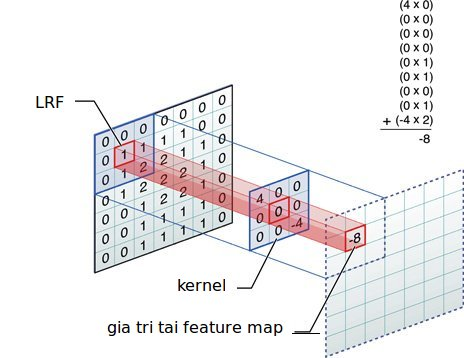
\includegraphics[scale=0.6]{parConv} 
    				\caption[Caption for LOF]{các thành phần quá trình tính toán tích chập.\protect\footnotemark}
    				\label{Conv4}
  			\end{center}
\end{figure}	

 	Giá trị tại mỗi ô trong ma trận filter có kích thước là $(F \times F \times D_1) + 1$ (cộng một ở đây là tham số ngưỡng của filter) sẽ tương ứng là trọng số của filter. Các giá trị này sẽ không đổi trong suốt quá trình dịch chuyển tính toán trên toàn bộ hình ảnh. Đây là một đặc tính quan trọng của CNN, bởi nó làm giảm thêm trọng số cần học cho quá trình huấn luyện mạng. Qua đó, ta có thể ước tính tổng số tham số cần học trong quá trình sử dụng Conv là $(F \times F \times D_1) \times K + K$ (ở đây cộng thêm k tham số ngưỡng của k filter). \par
 	



 Áp dụng vào ví dụ cụ thể ở hình \ref{ConvVD}, đầu vào là một ảnh màu với kích thước $(32 \times 32 \times 3)$ ($W_1 = H_1 = 32$ và $D_1 = 3$ chỉ giá trị của các kênh màu RGB). Với số lượng filter K = 6, trong đó mỗi filter có kích thước ($5 \times 5 \times 3$). F = 3 với bước di chuyển S = 1 và P = 0. Tương ứng với mỗi filter, ta thu được 6 feature map khác nhau ở đầu ra. trong đó:
 \begin{itemize}
 	\item $W_2 = \frac{32 - 5}{1} + 1 = 28$
 	\item $W_1 = \frac{32 - 5}{1} + 1 = 28$
 	\item $D_1 = 6$ 	
 \end{itemize}

	Mỗi neural trong một feature map sẽ có số tham số là $(F \times F \times D_1) = 5 \times 5 \times 3 + 1$. nếu không sử dụng tính chất shared weights thì tổng số tham số trong mạng cần phải học cho tất cả các feature map là $(28 \times 28 \times 6) \times (5 \times 5 \times 3 + 1) = 357504$ (tham số). Mặc dù con số đó đã nhỏ hơn nhiều so với việc không sử dụng Conv nhưng con số trên vấn lơn hơn rất nhiều so với $(F \times F \times D_1) \times K + K = (5 \times 5 \times 3) \times 6 + 6 = 456$ (tham số) khi sử dụng shared weights. \par
	
\begin{figure}[ht]
  			\begin{center}
    				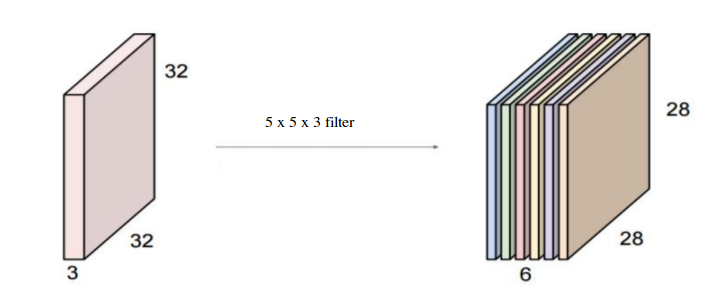
\includegraphics[scale=0.5]{ConvVD} 
    				\caption[Caption for LOF]{Ví dụ kết quả tính toán Conv trong hình ảnh.}
    				\label{ConvVD}
  			\end{center}
\end{figure}	

Nói tóm lại, Việc sử dụng Conv có những ưu điểm sau:
\begin{itemize}
	\item Giảm số lượng tham số: trong mạng ANN truyền, mỗi neural ở lớp trước sẽ liên kết tới tất cả các neural ở lớp kế tiếp (fully connected). Dẫn đến tình trạng số lượng các tham số trong mạng rất lớn. Đây là nguyên nhân chính gây việc thời gian huấn luyện mạng rất lâu. Với việc sử dung Conv, cho phép chia sẻ trọng số liên kết (shared weights), cũng như sử dụng LRF giúp cho số lượng các tham số trong mạng giảm đi đáng kể.
	\item Các tham số trong quá trình sử dụng Conv hay các giá trị trong các filter sẽ được học trong quá trình huấn luyện mạng. Sau quá trình tính toán, ta sẽ thu được các thông tin đặc trưng như góc, cạnh, Đốm màu trong ảnh, ... Chính vì thế, Conv còn có vai trò xây dựng mô hình tự học ra các đặc trưng.
\end{itemize}

\subsubsection{Lớp Pooling}
	Lớp Pooling được sử dụng đứng ngay sau convolution. Pooling giúp cho mạng giảm số lượng tham số, từ đó giúp đơn giản hóa quá trình tính toán của CNN và qua đó góp phần giải quyết vấn đề overfiting khi huấn luyện mạng. \par
	Có nhiều toán tử pooling như Sum-pooling, Max-pooling, L2-pooling nhưng Max-pooling được sử dụng phổ biến nhất trong kiến trúc mạng CNN vì nó cho kết quả hơn so với những toán tử còn lại. \par

\begin{figure}[ht]
  			\begin{center}
    				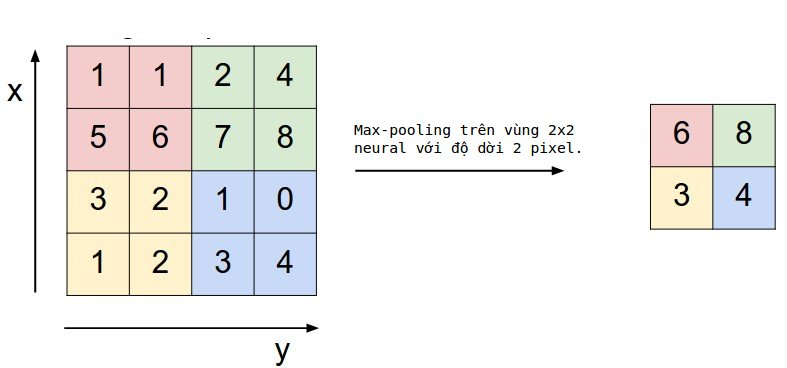
\includegraphics[scale=0.5]{maxpool} 
    				\caption{Max-pooling lấy giá trị lớn nhất trên vùng $[2\times2]$ trên kích thước $[4\times4]$ và thu được đầu ra kích thước $[2\times2]$.}
    				\label{maxpool}
  			\end{center}
\end{figure}	

	Ngoài ra, Max-pooling còn giúp tạo ra tính bất biến dịch chuyển (translation invatiance) cho đặc trưng. Cụ thể, dù đối tượng trong hình ảnh đầu vào có sự dịch chuyển nhỏ thì mạng vẫn có khả năng phân lớp chính xác được đối tượng. Đó là bởi vì max-pooling chọn ra neural có giá trị đầu ra tối ra tại mỗi vùng neural của lớp trước và tổng hợp thành lớp sau. Việc chọn neural có giá trị tín hiệu lớn nhất được xem như chọn ra đặc trưng tốt nhất để xử lý. Chính vì thế, khả năng phân lớp chính xác đối tượng dựa trên đặc trưng này vẫn không thay đổi và giúp cho CNN đạt được tính ổn định khi đối tượng di chuyển. \par
	Trong lớp Conv, có thể có nhiều feature map, tương ứng với mỗi feature map sẽ có một lớp max-pooling. Hình \ref{pooling} là một ví dụ minh họa, với lớp đầu vào kích thước $[28\times28]$ giả sử ta thu được ba feature map kích thước $[24\times24]$ và ba lớp max-pooling kích thước $[12\times12]$, ta sử dụng kernel kích thước $[5\times5]$ và max-pooling lấy giá trị lớn nhất tại mỗi vùng $[2\times2]$ neural. 
	
\begin{figure}[ht]
  			\begin{center}
    				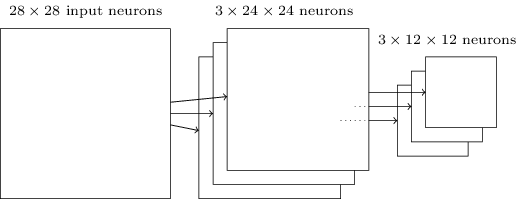
\includegraphics[scale=0.7]{pooling} 
    				\caption{Minh họa áp dụng Pooling từ lớp Conv}
    				\label{pooling}
  			\end{center}
\end{figure}	
	

\subsubsection{Lớp Normalization}
	Lớp Normalization (Norm) là lớp giúp chuẩn hóa dữ liệu đầu ra cho các lớp trong CNN trước khi được truyền đi tiếp. trong những kiến trúc CNN lớn và phức tạp, Lớp Norm sẽ chuẩn hóa các giá trị neural trước khi chúng được truyền đến hàm ReLU. Hàm ReLU tuy giúm rút ngắn thời gian huấn luyện, nhưng nếu không điều chỉnh trọng số phù hợp, hàm ReLU sẽ rất dễ gặp phải vấn đề "dying ReLU" khiến cho mạng trể nên chậm hơn khi huấn luyện. Lớp Norm lúc này sẽ chuẩn hóa và tạo ra các giá trị tích chập phù hợp để tránh cho ReLU rơi vào giá trị 0. Tránh việc gradient xấp xỉ bằng 0 khiến cho tốc độ học của mạng trở nên rất chậm.

\section{Áp dụng Deep Learning cho bài toán đếm đối tượng}
	Từ những kiến thức nền tảng đã trình bài ở hai phần trên, phần này sinh viên sẽ tiền hành trình bày một phương pháp áp dụng giải quyết cho bài toán đếm đối tượng. Cụ thể về chi tiết kỹ thuật và các mô hình được sử dụng để giải quyết bài toán. 
\subsection{Mô hình đếm đối tượng}
	Phươn pháp được sử dụng sau đây là một phương pháp thuộc nhóm Counting by Regression. Đầu tiên, Sinh viên sẽ trình bày mô hình tổng quát áp dụng cho bài toán, kèm theo đó là các ký hiệu và công thức tính toán được sử dụng. Đối với phương pháp này, ta định nghĩa lại bài toán đếm đối tượng thành mô hình bài toán ước lượng mật độ đối tượng (density estimation) được đề cập trong công trình của Victor and Zisserman \cite{lempitsky2010learning}. \par
	Quá trình huấn luyện của phương pháp này đòi hỏi cần phải có một tập các hình ảnh gán nhãn. Cụ thể hơn, tất cả các đối tượng trong tập hình ảnh huấn luyện sẽ được đánh dấu bằng một dấu chấm. Gỉa sử ta có một tập huấn luyện với N bức hình $I_1,I_2,I_3,...,I_N$, với mỗi bức hình $I_i$ ta có một tập các điểm đã được đánh dấu bằng các điểm 2 chiều (2D) $P_i = \{P_1,P_2,...,P_S\}$. Ở đây, S là tổng số lượng các nhãn (dấu chấm) đã được đánh dấu. \par
	Trong hướng tiếp cận này, ta sẽ sẽ dụng một hàm mật độ để tính toán ra những giá trị số thực biểu diễn cho giá trị của toàn bộ pixel trong bức hình, sao cho tất cả các giá trị này sẽ biểu diễn phù hợp nhất cho các đối tượng cần đếm. Cụ thể hơn, với một hình ảnh huấn luyện I. Trong quá trình tạo ra ground truth, ta định nghĩa một hàm tính mật độ nhằm tạo ra ground truth $D_I$ cho mỗi ảnh I, bằng việc sử dụng hàm Gaussian hai chiều cho mỗi điểm được đánh dấu.
\begin{align}
   \forall p \in I_i   \hspace{1cm}   D_i(p) = \displaystyle \sum_{p \in P_i} \mathcal{N}(p;P,\sigma^2 1_{2\times2})
\end{align}

	Ở đây, p đại diện cho pixel đang xử lý và $\mathcal{N}(p;P,\sigma^2 1_{2\times2})$   là hàm Gaussian hai chiều để ước lượng giá trị tại điểm p,  
	Từ bản đồ mật độ $D_I$ thu được, ta tính $N_I$ là tổng các đối tượng xuất hiện trong hình bằng cách tính tổng tất cả gác giá trị pixel trên toàn bộ $D_I$ theo công thức.
	 
\begin{align}\label{ct3} 
   N_I = \sum_{p \in I}D_I(P)
\end{align}

Bằng cách gán nhãn sử dụng dấu chấm cho mỗi đối tượng và tính tổng giá trị của hàm Gaussian trên toàn bộ pixel của ảnh. Vì thế tất cả các đối tượng sẽ được đếm một cách đầy đủ cả trong trường hợp những đối tượng bị chồng lấp lên nhau.\par

	Với mô hình bài toán ước lượng số lượng đối tượng, mục tiêu chính của phương pháp này chính là thiết kế ra một kiến trúc mô hình Deel Learning có khả năng học và tạo ra mộ hàm hồi quy phi tuyến tính (non-linear regression) $\mathcal{R}$. Cụ thể, $\mathcal{R}$ sẽ nhận đầu vào là một patch P của ảnh và sau khi xử lý sẽ cho ra một dự đoán ước lượng bản đồ mật độ $D_{pred}^{(P)}$
\begin{align}
   D_{pred}^{(P)} = \mathcal{R}(P|\Omega)
\end{align}
	Trong đó $\Omega$ là tập các tham số của mô hình CNN sử dụng. Với mỗi patch hình ảnh $P \in \mathbb{R} ^ { h \times w \times c}$, trong đó h và w là chiều cao và chiều rộng, c là số kênh màu của patch ảnh. Và kết quả thu được là $D_{pred}^{(P)} \in \mathbb{R} ^ { h' \times w'} $, trong đó h' và w' lần lượt là chiều cao và chiều rộng của bản đồ mật độ sau khi tính toán. Như vậy, với một hình ảnh đầu vào, đầu tiền ta sẽ tiến hành rút ra những patch của nó, sau đó mô hình CNN sẽ xử lý và cho ra một bản đồ mật độ tương ứng với mỗi patch. và cuối cùng ta sẽ tích hợp tất cả các bản đồ mật độ thu được để cho ra density map của toàn bộ bức hình (minh họa trong hình \ref{mohinh}). Sau đây, sinh viên sẽ trình bày chi tiết kiến trúc mô hình CNN sử dụng trong mô hình này.
	
\begin{figure}[ht]
  			\begin{center}
    				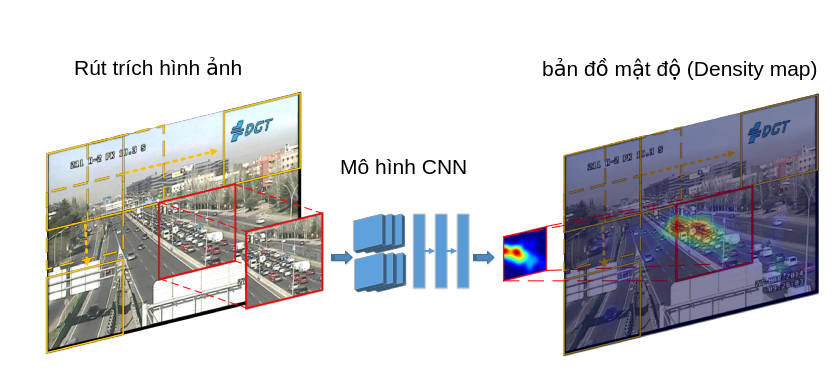
\includegraphics[scale=0.5]{mohinh} 
    				\caption{Mô hình giải quyết bài toán đếm đối tượng với đầu vào là một bức ảnh và đầu ra là một bản đồ mật độ đối tượng trong bức ảnh đó.} 
    				\label{mohinh}
  			\end{center}
\end{figure}	




\subsection{Mô hình CCNN}
	Trong phần này, sinh viên sẽ trình bày kiến trúc CNN đầu tiên được sử dụng, mô hình Counting Convolutional Neural Networks (CCNN). Kiến trúc của mô hình CCNN bao gồm 6 lớp Convolituonal. Lớp Conv1 và Conv2 sử dụng kernel với kích thước $7 \times 7$ cùng chiều sâu là 32. Lớp Conv3 chứa kernel $5 \times 5$ cùng chiều sâu 64 và sau đó kết nối với lớp max-pooling có kernel kích thước $2 \times 2$. Conv4 và Conv5 chứa kernel kích thước $1 \times 1$ với chiều sâu tương ứng lần lượt là 1000 và 400. \par 
	Như đã trình bày trong công thức \eqref{ct3}, mô hình này đề xuất một mô hình học phi tuyến tính (non-linear) đề có thể biểu diễn các đối tượng trong bức ảnh thành một bản đồ mật độ phù hợp với nó. Chính vì thế, ta sẽ huấn luyện mô hình CCNN để giải quyết bài toán này theo lớp bài toán regression. Đề làm được điều này, ta cần kết nối lớp Conv6 với một hàm mất  
\subsection{Mô hình Hydra CNN}
\section{Kết chương}


